\section{The Simulation}
In contrast to the large scale threshold analysis done by \citet{OGorman2016} this work focusses on the physical simulation of the building block of the surface code error detection - the stabilizer measurements which is done by measuring the parity of a group of qubits. On the smallest scale this is given by a group of four data qubits and one probe/ancillary qubit as shown in 
The interaction is governed by the following Hamiltonian:

\begin{equation}
H = \mu_B B( g_1 \sigma_1^Z + g_2 \sigma_2^Z) + \frac{J}{r^3} ( \mathbf{\sigma_1} \cdot \mathbf{\sigma_2} - 3 ( \hat{\mathbf{r}} \cdot \mathbf{\sigma_1}) ( \hat{\mathbf{r}}\cdot \mathbf{\sigma_2}))
\end{equation}
The effect of this Hamiltonian is to evolve the probe qubit in a particular direction depending on the state of the data qubit. By initialising the probe qubit in the $\ket{+}$ state, the final parity measurement will entail finding the probe qubit in either the $\ket{+}$ state (even parity) or in the $\ket{-}$ state. This can be understood by the fact that each data qubit imparts a $\frac{\pi}{2}$ phase in 

\subsection{Finding the correct evolution time}
The speed of the simulation is set by the total time it takes to complete one full cycle. We want the accumulated phase for an even parity measurement to reach $2\pi$ exactly. The plot in Figure \ref{fig:plot} shows the accumulated phase as a function of evolution time. 



\begin{figure}[H]
	\subfloat[]{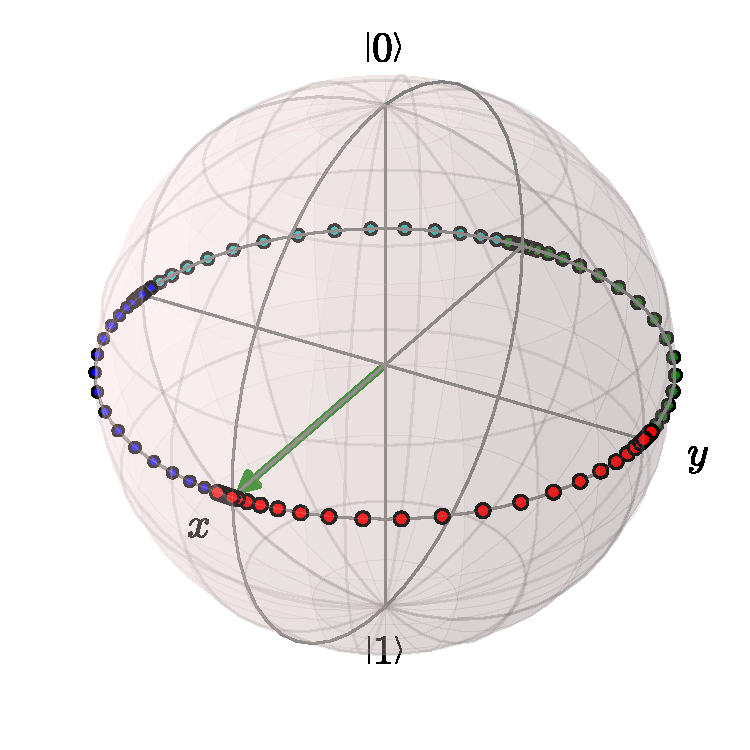
\includegraphics[width=0.49\linewidth]{../Figures/perfect_evolution_even} \label{FIG:even}}
	\subfloat[]{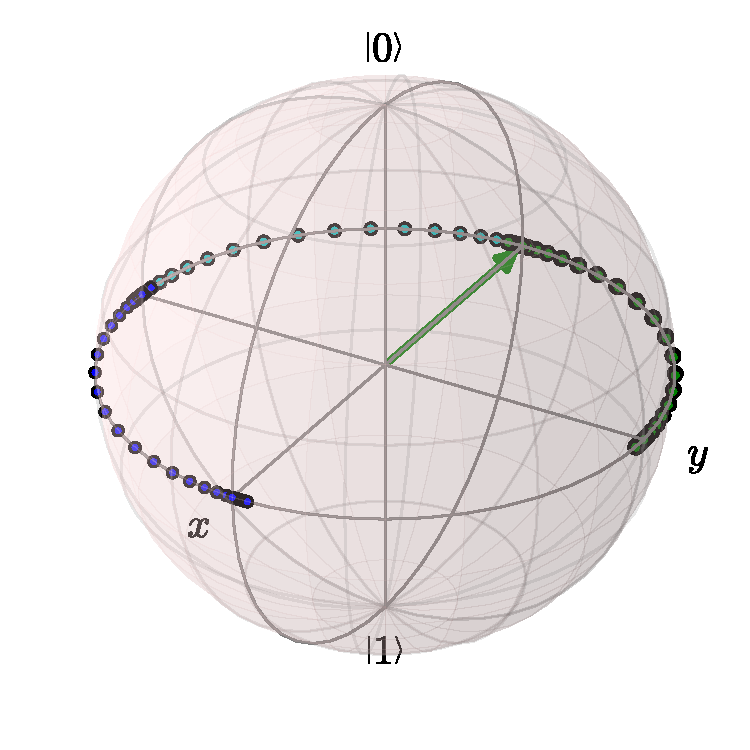
\includegraphics[width=0.49\linewidth]{../Figures/perfect_evolution_odd} \label{FIG:odd}}
	\caption[oddeven]{}
	\label{FIG:evolution}
\end{figure}


\begin{figure}[H]
	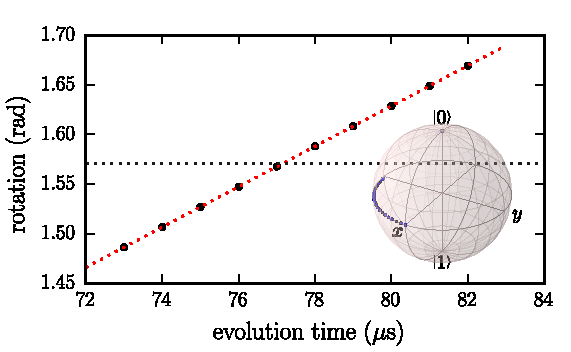
\includegraphics[width=\linewidth]{../Figures/abrupt_find_tau_full.pdf}
		\caption{}
		\label{fig:abrupt_tau}

\end{figure}


\begin{figure}[H]
	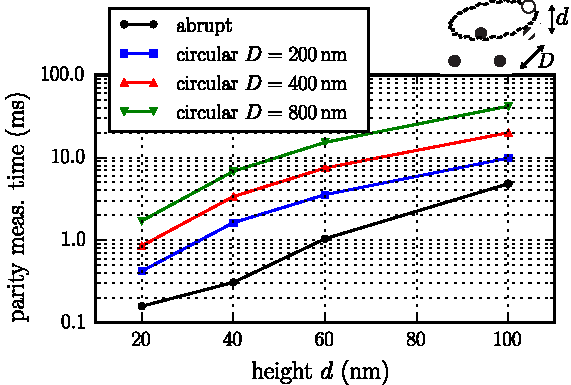
\includegraphics[width=\linewidth]{../Figures/tau_d_D}
	\caption{}
	\label{FIG:tau}
\end{figure}
